% !TeX program = xelatex
% !TeX encoding = UTF-8
% Generated from manuscript.md by build.py; edit the Markdown source.
\documentclass[12pt,a4paper]{article}
\usepackage{fontspec,amsmath,unicode-math}
\usepackage[main=russian,english]{babel}
\usepackage[top=20mm,bottom=25mm,left=30mm,right=10mm]{geometry}
\usepackage{setspace,graphicx,array,longtable,ragged2e,xurl,titlesec}
\titleformat{\section}{\fontsize{14}{17}\selectfont\bfseries\raggedright\hyphenpenalty=10000}{}{0em}{}
\titleformat{\subsection}{\fontsize{12}{15}\selectfont\bfseries\raggedright\hyphenpenalty=10000}{}{0em}{}
\setmainfont{Times New Roman}
\setmathfont{TeX Gyre Termes Math}
\urlstyle{same}
\doublespacing
\setlength{\emergencystretch}{3em}
\setlength{\parindent}{1.25cm}
\begin{document}
\noindent УДК 612.8:004.942\par
\begin{center}\bfseries\fontsize{14}{17}\selectfont Коннектомно-ограниченное предобучение для биофизического моделирования вызванных составных потенциалов действия при стимуляции спинного мозга: предпосылки и критерии проверки\end{center}
\section*{Аннотация}
Коннектомные модели позволяют исследовать связь анатомической структуры с динамикой нейронных систем, однако их использование для предобучения моделей человеческих электрофизиологических сигналов требует отдельного обоснования. В критическом нарративном обзоре сопоставлены исследования нейродинамики Drosophila, ноцицептивных цепей, обучения представлений и биофизического моделирования вызванных составных потенциалов действия при стимуляции спинного мозга. Цель работы — определить проверяемые предпосылки переноса и условия, при которых его предполагаемая польза может быть оценена без отождествления процессов разных видов. Основной целевой задачей выбрано моделирование кривой роста амплитуды регистрируемого ответа. Предложена формальная схема, в которой переносится начальная параметризация временного модуля, а человеческое рекрутирование волокон и регистрация сигнала описываются отдельными компонентами. Результат литературного сопоставления представлен доказательной матрицей четырёх связей: коннектом и динамика; динамика и представление; рекрутирование и измеряемый сигнал; предобучение и дополнительная техническая ценность. Для каждой связи определены доступные основания, ограничения и необходимая проверка. Рассмотрены контрольные условия, позволяющие разделить эффекты топологии, обученной динамики, источника предобучения и физического оператора. Основным показателем предложена средняя межучастническая ошибка амплитуды кривой роста, рассчитанная предварительно для каждого участника. Практически значимое преимущество, достаточно точно установленное отсутствие преимущества, ухудшение и неопределённый результат рассматриваются раздельно. До независимой проверки оператора вычислительный результат обозначается как ECAP-подобный сигнал. Литература обосновывает изучение отдельных компонентов, но не устанавливает пользу переноса Drosophila для данной задачи. Предлагаемая схема определяет предмет будущего сравнения, требования к данным и границы допустимого вывода; экспериментальные результаты переноса в работе не заявляются.\par
\noindent\begin{minipage}{\linewidth}Ключевые слова: коннектом, Drosophila, предобучение, временное представление, вызванный составной потенциал действия, стимуляция спинного мозга, биофизическая модель, валидация.\end{minipage}\par
\section*{Введение}
Вызванный составной потенциал действия (ECAP) отражает суммарный электрический ответ рекрутированных нервных волокон. При стимуляции спинного мозга (SCS) зависимость амплитуды ответа от интенсивности воздействия — кривая роста — используется для характеристики измерительного канала. Её изменение определяется не только рекрутированием, но и геометрией регистрации, положением тела и параметрами импульса [1–3]. Пороги восприятия, сопоставляемые с ECAP, не являются показателями обезболивания [4].\par
Предобучение временного модуля на динамике коннектомной модели Drosophila представляет возможный способ задания начальных параметров. Его дополнительная ценность относительно человеческой биофизической модели и простой кривой роста не установлена. Предмет обзора — основания и критерии проверки этой гипотезы; анатомическое соответствие мухи и спинного мозга человека не предполагается.\par
\section*{Материалы и методика}
Выполнен критический нарративный обзор. Исходный тематический отбор включал 20 работ; их роль и ограничения пересмотрены отдельно от дополнения. 5 октября 2026 года в PubMed и Crossref применены десять англоязычных запросов: по два для коннектомной динамики, ноцицепции, переноса представлений, физического моделирования ECAP и измерения либо управления SCS. Дополнительно применены два русскоязычных запроса. Период дополнения — с 2015 года до даты поиска. Для каждого запроса просмотрены первые 20 результатов в порядке релевантности либо вся меньшая выдача; точные запросы, ранги и решения сохранены в сопроводительном реестре.\par
Включались работы, раскрывающие механизм одного из четырёх рассматриваемых звеньев, его ограничения или условия проверки. Дубликаты, рецензии как отдельные поисковые записи, непрофильные задачи и повторные клинические описания исключались. Отдельно добавлены первичная публикация взрослого коннектома и патентный аналог. Отобраны 24 источника. Полные тексты и доступные разделы сопоставлялись с исходными локаторами; для частичных текстов использованы только явно доступные сведения. Полнота систематического поиска и отсутствие всех возможных аналогов не заявляются. Русскоязычное дополнение не выявило в просмотренной выдаче непосредственно подходящих работ; это ограничение двух запросов, а не вывод об отечественной литературе в целом.\par
\section*{Результаты литературного сопоставления}
\subsection*{Основания и границы источников}
\begin{longtable}{|>{\RaggedRight\hyphenpenalty=50\exhyphenpenalty=50\arraybackslash}p{\dimexpr 0.29\linewidth-2\tabcolsep-1.3333333333333333\arrayrulewidth\relax}|>{\RaggedRight\hyphenpenalty=50\exhyphenpenalty=50\arraybackslash}p{\dimexpr 0.32\linewidth-2\tabcolsep-1.3333333333333333\arrayrulewidth\relax}|>{\RaggedRight\hyphenpenalty=50\exhyphenpenalty=50\arraybackslash}p{\dimexpr 0.39\linewidth-2\tabcolsep-1.3333333333333333\arrayrulewidth\relax}|}
\multicolumn{3}{@{}p{\linewidth}@{}}{Таблица 1. Включённые источники, проверенный результат и граница вывода. П — журнальная публикация; Пр — препринт. Полный текст означает доступность текста и проверку относящихся к выводу разделов, а не независимое воспроизведение работы.\par \foreignlanguage{english}{Table 1. Included sources, reviewed results and limits. J: journal publication; P: preprint. Available full text denotes reading the relevant sections, not independent reproduction.}\par} \\ \hline
\textbf{Источник; версия и доступ} & \textbf{Результат для сопоставления} & \textbf{Ограничение} \\ \hline
\endfirsthead
\hline
\textbf{Источник; версия и доступ} & \textbf{Результат для сопоставления} & \textbf{Ограничение} \\ \hline
\endhead
\endfoot
\endlastfoot
[1]; П, полный текст & Поза и ширина импульса изменяют ECAP & Постоянная амплитуда не гарантирует постоянное рекрутирование; не прогноз боли \\ \hline
[2]; П, полный текст & Вычислительная оценка направленных электродов & Нет независимой участнической проверки \\ \hline
[3]; П, полный текст & Последовательное моделирование возбуждения и регистрации & Упрощённая анатомия; пороги восприятия заданы предположениями \\ \hline
[4]; П, полный текст & ECAP и пороги восприятия у 14 участников & 112 кривых — повторные измерения; не исход обезболивания \\ \hline
[5]; П, полный текст & Восстановление динамики при коннектомных ограничениях & Эталонная сеть вычислительная, не биологическая \\ \hline
[6]; П, полный текст & Проверка отдельных сенсомоторных цепей взрослой мухи & Абсолютные частоты модели ограниченно интерпретируемы \\ \hline
[7]; П, полный текст & Разные механизмы острой ноцицепции и гиперчувствительности & Личинка; защитное поведение не субъективная боль \\ \hline
[8]; П, полный текст & Нисходящее торможение времени защитной реакции & Нет межвидового переноса \\ \hline
[9]; Пр 2025, номер версии не установлен & Восходящие пути взрослой мухи и избегание & Стадия и воздействие отличны от личиночных исследований \\ \hline
[10]; Пр v3, проверенные разделы & Совместное рассмотрение анатомии и кальциевых ответов & Возрастные группы и наблюдаемые величины различаются \\ \hline
[11]; Пр v2, полный текст & Кольцевой аттрактор и кальциевые наблюдения & Направление головы, не ноцицепция \\ \hline
[12]; Пр v1, проверенные разделы & Динамика двигательной сети & Без тела и обратной связи; нет проверки фаз по регистрации \\ \hline
[13]; Пр v1, проверенные разделы & Контроли инициализации и переподключения графа & Вывод зависит от задачи и метрики \\ \hline
[14]; Пр v1, проверенные разделы & Латентное представление графа для резервуарных задач & Коннектом мыши; нет ECAP \\ \hline
[15]; П, полный текст & Синтетические данные и адаптация для оценки боли & Неразмеченные данные тестовых участников входят в адаптацию \\ \hline
[16]; П, проверенные разделы & Признаки ECAP восьми выбранных участников & Проверка по сигналам, а не по исключённым участникам \\ \hline
[17]; П, проверенные разделы & Модель удаления артефакта & Два участника; неоднозначность определения итоговой метрики \\ \hline
[18]; П с исправлением, полный текст & Техническая осуществимость автоматизированного программирования & Исходы обезболивания не собирались \\ \hline
[19]; П с исправлением, аннотация и проверенные сведения & Клиническое сравнение EVOKE, 24 месяца & Вторичный анализ; не новая независимая когорта \\ \hline
[20]; П, полный текст & Клиническое сравнение EVOKE, 36 месяцев & Та же когорта; анализ 36 месяцев не предзадан \\ \hline
[21]; П, полный текст & FlyVis: обучение неизвестных параметров и прогноз зрительных ответов & Зрительная задача; не перенос к человеку \\ \hline
[22]; П, полный текст & Коннектом мозга взрослой самки & Структура не задаёт единственную динамику; не ресурс личинки \\ \hline
[23]; патент, описание и формула & Синтетические ECAP и предобучение классификатора & Раскрытие способа не подтверждает эффективность \\ \hline
[24]; П, первичная аннотация & Артефакты могут имитировать нейронный ответ & Свинья; вывод ограничен доступной аннотацией \\ \hline
\end{longtable}\par\smallskip
Коннектом ограничивает структуру модели, но оставляет неопределёнными динамические параметры. FlyVis показывает пользу сочетания анатомии и оптимизации для конкретной зрительной задачи [21]; вычислительная идентифицируемость [5] и результаты контролей топологии [13] не превращают этот частный результат в универсальный закон. Публикация взрослого мозга [22] описывает анатомический ресурс, который следует отличать от программного доступа к его данным.\par
В личиночной работе [10] число синапсов и знаки взаимодействий используются как ограничения, а кальциевые ответы — для сопоставления результатов. Возраст, версия графа, способ стимуляции и функция наблюдения должны согласовываться отдельно. Личиночные цепи [7, 8, 10], взрослые пути [9] и динамика ориентации либо ходьбы [11, 12] не образуют одну экспериментальную систему.\par
Синтетическое обучение и адаптация [14, 15] служат методическими аналогами. В работе [15] отсутствие тестовых меток не означает отсутствия тестовых участников в неразмеченной адаптации; авторы признают возможную оптимистическую оценку. В [16] внешнее разбиение выбирает каждый одиннадцатый сигнал, а не исключает участника. Эти работы не подтверждают межучастническое обобщение предлагаемой модели.\par
Для [18] учтено исправление названия сравнительного метода на Artefact Model Method. В [19] учтена перестановка обозначений групп в панели 4C; её значения здесь не воспроизводятся. Техническая регистрация, пользовательский опыт и клинические исходы различаются. Продолжения EVOKE [19, 20] не являются независимыми репликациями. Патент [23] исключает трактовку самого сочетания синтетических ECAP и предобучения как установленной новизны предлагаемой схемы.\par
\subsection*{Формальная схема переноса}
Источник задаётся графом \ensuremath{G_{F}}, воздействием \ensuremath{u_{F}} и динамикой \ensuremath{x_{F}}. Исходный адаптер \ensuremath{P_{F}} переводит выбранные наблюдения в вход временного модуля \ensuremath{E_{\omega}}; исходная обучающая задача определяет его параметры ω₀. Для человеческого канала применяются отдельный адаптер \ensuremath{P_{H}} и компонент рекрутирования \ensuremath{B_{\alpha}}. Оператор \ensuremath{H_{\varphi}} описывает проведение, суммирование и регистрацию при заданной геометрии. Индексы F и H обозначают вид, а не соответствие анатомических узлов.\par
\[x^F_{t+1}=F_{\theta_F}(x^F_t,u^F_t;G_F),\quad z^F_t=E_\omega(P_F(x^F_{\leq t},u^F_{\leq t}))\]
\[r^H_t=B_\alpha(E_\omega(P_H(u^H_{\leq t}))),\quad y^H(t)=H_\varphi(r^H)(t)\]
Переносятся только начальные параметры ω₀ временного модуля. Граф \ensuremath{G_{F}}, исходные состояния, исходный адаптер и параметры человеческого оператора не переносятся. Компонент \ensuremath{B_{\alpha}} выдаёт допустимые вероятности или характеристики рекрутирования \ensuremath{r_{H}}; их ограничения должны согласовываться с выбранной моделью волокон. Возбуждение рассчитывается в этом компоненте один раз. \ensuremath{H_{\varphi}} получает уже определённое рекрутирование и не повторяет его вычисление. Артефакт измерения моделируется отдельно от нейронного вклада.\par
\begin{center}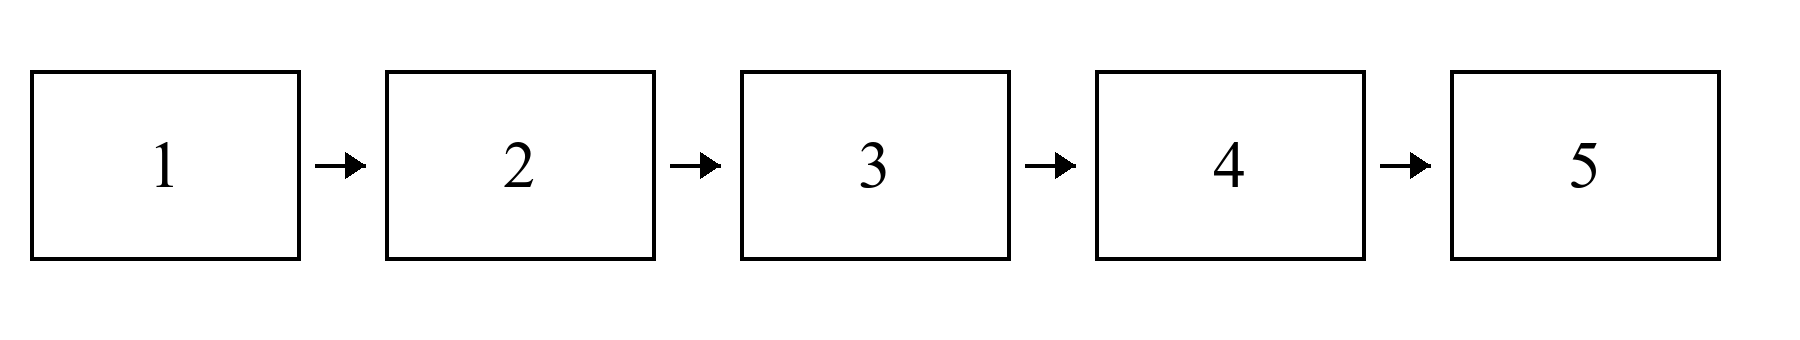
\includegraphics[width=0.96\linewidth]{figures/transfer-scheme.png}\end{center}
Рисунок 1. Схема предлагаемой проверки: 1 — динамика мухи и исходный адаптер; 2 — предобучение временного модуля; 3 — целевой адаптер и рекрутирование человека; 4 — оператор регистрации; 5 — ECAP-подобный сигнал и кривая роста. Стрелка между 2 и 3 обозначает перенос начальных параметров, а не анатомии.\par
\foreignlanguage{english}{Figure 1. Proposed evaluation scheme: 1, fly dynamics and source adapter; 2, temporal module pretraining; 3, target adapter and human recruitment; 4, recording operator; 5, ECAP-like signal and growth curve. The arrow from 2 to 3 transfers initial parameters, not anatomy.}\par
Модуль \ensuremath{E_{\omega}} обрабатывает историю входа; его внутреннее состояние обновляется рекуррентно либо эквивалентным временным преобразованием. Архитектура временного модуля не фиксируется. Необходимость памяти должна проверяться относительно простой модели кривой роста без временного состояния. Если вход представлен только интенсивностью одиночного импульса, дополнительная память может быть избыточна. История стимуляции и восстановление возбудимости дают возможную постановку временной задачи, но её наличие в доступных данных ещё требуется установить.\par
\begin{longtable}{|>{\RaggedRight\hyphenpenalty=50\exhyphenpenalty=50\arraybackslash}p{\dimexpr 0.22\linewidth-2\tabcolsep-1.3333333333333333\arrayrulewidth\relax}|>{\RaggedRight\hyphenpenalty=50\exhyphenpenalty=50\arraybackslash}p{\dimexpr 0.47\linewidth-2\tabcolsep-1.3333333333333333\arrayrulewidth\relax}|>{\RaggedRight\hyphenpenalty=50\exhyphenpenalty=50\arraybackslash}p{\dimexpr 0.31\linewidth-2\tabcolsep-1.3333333333333333\arrayrulewidth\relax}|}
\multicolumn{3}{@{}p{\linewidth}@{}}{Таблица 2. Сопоставимые свойства и статус предположений.\par \foreignlanguage{english}{Table 2. Comparable properties and hypothesis status.}\par} \\ \hline
\textbf{Свойство} & \textbf{Условие сопоставления} & \textbf{Статус} \\ \hline
\endfirsthead
\hline
\textbf{Свойство} & \textbf{Условие сопоставления} & \textbf{Статус} \\ \hline
\endhead
\endfoot
\endlastfoot
Вход и наблюдение & Воздействие и выбранная активность мухи; история стимуляции и рекрутирование человека & Разные физические величины; общий закон не установлен \\ \hline
Размерность & Раздельные адаптеры в пространство размерности k & Авторский способ согласования, не анатомическое тождество \\ \hline
Время & Отдельные шаги и окна; масштаб определяется на обучающих данных & Кальциевый сигнал и электрический ответ нельзя приравнять \\ \hline
Нормировка & Отдельно по видам и обучающим разбиениям; выход в микровольтах & Нормировка сама по себе не доказывает сходство \\ \hline
Переносимое свойство & Предсказательная структура отклика на историю входа & Гипотеза; при отсутствии основания заявка прекращается \\ \hline
\end{longtable}\par\smallskip
\subsection*{Проверки, вытекающие из литературы}
\begin{longtable}{|>{\RaggedRight\hyphenpenalty=50\exhyphenpenalty=50\arraybackslash}p{\dimexpr 0.23\linewidth-2\tabcolsep-1.3333333333333333\arrayrulewidth\relax}|>{\RaggedRight\hyphenpenalty=50\exhyphenpenalty=50\arraybackslash}p{\dimexpr 0.24\linewidth-2\tabcolsep-1.3333333333333333\arrayrulewidth\relax}|>{\RaggedRight\hyphenpenalty=50\exhyphenpenalty=50\arraybackslash}p{\dimexpr 0.53\linewidth-2\tabcolsep-1.3333333333333333\arrayrulewidth\relax}|}
\multicolumn{3}{@{}p{\linewidth}@{}}{Таблица 3. Четыре звена доказательной схемы.\par \foreignlanguage{english}{Table 3. Four links of the evidence and evaluation scheme.}\par} \\ \hline
\textbf{Звено} & \textbf{Основание} & \textbf{Необходимая проверка и граница} \\ \hline
\endfirsthead
\hline
\textbf{Звено} & \textbf{Основание} & \textbf{Необходимая проверка и граница} \\ \hline
\endhead
\endfoot
\endlastfoot
Коннектом → динамика & [5, 6, 10, 21, 22] & Совместимые граф и наблюдения; контроли инициализации и степеней [13] \\ \hline
Динамика → представление & [11, 12, 14] & Предсказание исходных наблюдений; исключение утечки и сравнение динамических контролей \\ \hline
Рекрутирование → сигнал & [1–3, 17, 24] & Независимая проверка регистрации и артефактов; возбуждение не дублируется \\ \hline
Предобучение → ценность & Методические аналоги [15, 16, 23] & Независимые участники и обязательные контроли; польза пока не установлена \\ \hline
\end{longtable}\par\smallskip
\begin{longtable}{|>{\RaggedRight\hyphenpenalty=50\exhyphenpenalty=50\arraybackslash}p{\dimexpr 0.35\linewidth-2\tabcolsep-1.3333333333333333\arrayrulewidth\relax}|>{\RaggedRight\hyphenpenalty=50\exhyphenpenalty=50\arraybackslash}p{\dimexpr 0.24\linewidth-2\tabcolsep-1.3333333333333333\arrayrulewidth\relax}|>{\RaggedRight\hyphenpenalty=50\exhyphenpenalty=50\arraybackslash}p{\dimexpr 0.41\linewidth-2\tabcolsep-1.3333333333333333\arrayrulewidth\relax}|}
\multicolumn{3}{@{}p{\linewidth}@{}}{Таблица 4. Контрольные условия будущего сравнения.\par \foreignlanguage{english}{Table 4. Control conditions for a future comparison.}\par} \\ \hline
\textbf{Условие} & \textbf{Проверяемый эффект} & \textbf{Требование} \\ \hline
\endfirsthead
\hline
\textbf{Условие} & \textbf{Проверяемый эффект} & \textbf{Требование} \\ \hline
\endhead
\endfoot
\endlastfoot
Простая кривая роста без памяти & Необходимость временного модуля & Те же входные сведения и разбиения \\ \hline
Человеческая модель без предобучения & Эффект переноса & Сопоставимые размерность и бюджет настройки \\ \hline
Предобучение на человеческих синтетических ECAP & Выбор исходного домена & Тот же оператор и доступные данные \\ \hline
Неноцицептивная динамика мухи & Специфичность источника & Сопоставимый объём и задача обучения \\ \hline
Перемешанное время & Польза временной организации & Сохранение распределения входов \\ \hline
Переподключённый граф & Польза топологии & Сохранение степеней и общая инициализация \\ \hline
Топология без обученной динамики & Структура и обучение & Раздельная оценка вклада параметров \\ \hline
Замороженный и дообучаемый модуль & Адаптация параметров & Общие разбиения; настройки внутри обучения \\ \hline
Модель без оператора регистрации & Нефизический обход задачи & Только диагностический контроль \\ \hline
\end{longtable}\par\smallskip
Факторы могут проверяться в последовательных сопоставлениях; полный набор всех комбинаций не предписывается. Выбор основного и независимого человеческих наборов пока не сделан. Требуются участнические идентификаторы, параметры стимуляции, пригодные кривые роста, геометрия регистрации и разрешение на использование.\par
Для участника i основная предложенная ошибка \ensuremath{E_{i}} — RMSE амплитуды кривой роста в микровольтах. Итог E — среднее \ensuremath{E_{i}} по участникам, независимо от числа повторных сигналов. Преимущество Δ определяется как ошибка контроля минус ошибка переноса.\par
\[E_i=\sqrt{\frac{1}{m_i}\sum_j(\widehat A_{ij}-A_{ij})^2},\quad E=\frac{1}{N}\sum_i E_i,\quad\Delta=E_{\mathrm{control}}-E_{\mathrm{transfer}}\]
Здесь \ensuremath{A_{ij}} и \ensuremath{\widehat{A}_{ij}} — зарегистрированная и прогнозируемая амплитуды в j-й точке кривой участника i; \ensuremath{m_{i}} — число сопоставимых точек, N — число участников.\par
Повторные импульсы, сеансы и конфигурации не увеличивают число независимых участников. Определение амплитуды, окна, масштабы времени, калибровка и подбор параметров фиксируются внутри обучающих разбиений. Допуски практически значимого различия, объём выборки и статистический протокол определяются после проверки пригодности данных, до доступа к окончательной тестовой выборке. Форма, латентность и устойчивость регистрации остаются дополнительными характеристиками.\par
\section*{Обсуждение}
Авторский результат обзора — схема сопоставления доказательств и проверяемая постановка переноса. Она не доказывает эффективность метода. Практически значимое преимущество требует превышения заранее заданного порога с достаточной точностью; подтверждённое отсутствие преимущества — достаточно точной оценки относительно этого порога. Ухудшение и неопределённость рассматриваются отдельно. Широкий интервал оценки или недоступность данных не опровергают гипотезу.\par
Соответствующая заявка прекращается при отсутствии обоснованного сопоставимого свойства, несовместимости исходных наблюдений, непроверенном человеческом операторе или отсутствии пригодных человеческих данных. До независимой проверки вычислительный выход называется ECAP-подобным сигналом. При отсутствии данных допустимы отдельные модельные исследования, но не заявления о человеческой валидации.\par
Обзор ограничен тематическим исходным отбором, коротким поисковым дополнением, частичными текстами и наличием препринтов. Сходство латентных признаков не устраняет различий наблюдения. Ноцицептивное поведение мухи, субъективная боль, ECAP и клинический исход остаются разными конструкциями. Техническое преимущество в кривой роста не даёт основания обещать настройку лечения или обезболивание.\par
\section*{Заключение}
Литература поддерживает раздельное исследование коннектомных моделей и биофизического измерительного канала SCS. Дополнительная ценность предобучения на динамике Drosophila для кривой роста ECAP остаётся гипотезой. Предложены переносимый блок параметров, интерфейс рекрутирования и регистрации, доказательная матрица, контрольные условия и участническая метрика. Эти элементы позволяют определить, какое будущее сравнение будет информативным и при каких условиях заявка на перенос должна быть ограничена либо прекращена.\par
\section*{Список литературы}
\noindent\foreignlanguage{english}{1. Evoked compound action potentials during spinal cord stimulation: effects of posture and pulse width on signal features and neural activation within the spinal cord / Brucker-Hahn M.K., Zander H.J., Will A.J., Vallabh J.C., Wolff J.S., Dinsmoor D.A., Lempka S.F. Journal of Neural Engineering. 2023. Vol. 20. No. 4. Art. 046028. DOI: \url{10.1088/1741-2552/aceca4}.}\par
\noindent\foreignlanguage{english}{2. Directional leads applied to spinal cord stimulation: A computational modelling study / Wu Z., Wu N., Wang P., Zhang C., Wu C., Huo X., Zhang G. PLOS One. 2026. Vol. 21. No. 4. Art. e0345287. DOI: \url{10.1371/journal.pone.0345287}.}\par
\noindent\foreignlanguage{english}{3. Evoked Potentials Recorded From the Spinal Cord During Neurostimulation for Pain: A Computational Modeling Study / Anaya C.J., Zander H.J., Graham R.D., Sankarasubramanian V., Lempka S.F. Neuromodulation: Technology at the Neural Interface. 2020. Vol. 23. No. 1. P. 64–73. DOI: \url{10.1111/ner.12965}.}\par
\noindent\foreignlanguage{english}{4. The Evoked Compound Action Potential as a Predictor for Perception in Chronic Pain Patients: Tools for Automatic Spinal Cord Stimulator Programming and Control / Pilitsis J.G., Chakravarthy K.V., Will A.J., Trutnau K.C., Hageman K.N., Dinsmoor D.A., Litvak L.M. Frontiers in Neuroscience. 2021. Vol. 15. Art. 673998. DOI: \url{10.3389/fnins.2021.673998}.}\par
\noindent\foreignlanguage{english}{5. Beiran M., Litwin-Kumar A. Prediction of neural activity in connectome-constrained recurrent networks. Nature Neuroscience. 2025. Vol. 28. No. 12. P. 2561–2574. DOI: \url{10.1038/s41593-025-02080-4}.}\par
\noindent\foreignlanguage{english}{6. A Drosophila computational brain model reveals sensorimotor processing / Shiu P.K., Sterne G.R., Spiller N., Franconville R., Sandoval A., Zhou J., Simha N., Kang C.H., Yu S., Kim J.S., Dorkenwald S., Matsliah A., Schlegel P., Yu S.-C., McKellar C.E., Sterling A., Costa M., Eichler K., Bates A.S., Eckstein N., Funke J., Jefferis G.S.X.E., Murthy M., Bidaye S.S., Hampel S., Seeds A.M., Scott K. Nature. 2024. Vol. 634. No. 8032. P. 210–219. DOI: \url{10.1038/s41586-024-07763-9}.}\par
\noindent\foreignlanguage{english}{7. Nociception and hypersensitivity involve distinct neurons and molecular transducers in Drosophila / Gu P., Wang F., Shang Y., Liu J., Gong J., Xie W., Han J., Xiang Y. Proceedings of the National Academy of Sciences. 2022. Vol. 119. No. 12. Art. e2113645119. DOI: \url{10.1073/pnas.2113645119}.}\par
\noindent\foreignlanguage{english}{8. Feedback inhibition by a descending GABAergic neuron regulates timing of escape behavior in Drosophila larvae / Zhu J., Boivin J.-C., Garner A., Ning J., Zhao Y.Q., Ohyama T. eLife. 2024. Vol. 13. Art. RP93978. DOI: \url{10.7554/eLife.93978}.}\par
\noindent\foreignlanguage{english}{9. Ascending nociceptive pathways drive rapid escape and sustained avoidance in adult Drosophila / Jones J.M., Sustar A., Mamiya A., Walling-Bell S., Chou G.M., Cook A.P., Tuthill J.C. bioRxiv preprint. 2025. Preprint. bioRxiv, posted 2025-10-29. DOI: \url{10.1101/2025.10.28.684868}.}\par
\noindent\foreignlanguage{english}{10. Combining brain-wide activity imaging with electron microscopy reveals a distributed brain network for processing threatening somatosensory stimuli / Randel N., Wang C., Clayton M.S., Wang K., Pang S., Xu C.S., Champion A.S., Hess H.F., Cardona A., Keller P.J., Zlatic M. bioRxiv. 2026. Preprint. bioRxiv v3, posted 2026-08-03. DOI: \url{10.1101/2025.09.25.678485}.}\par
\noindent\foreignlanguage{english}{11. Biswas T., Stanoev A., Romani S., Fitzgerald J.E. From the fly connectome to exact ring attractor dynamics. bioRxiv. 2026. Preprint. bioRxiv v2, posted 2026-03-08. DOI: \url{10.1101/2024.11.01.621596}.}\par
\noindent\foreignlanguage{english}{12. How much of fly walking is written in the wiring? / Guan I., Zhao Y., Zhang D., Lyu S., Chen I.-M. arXiv. 2026. Preprint. arXiv:2609.38665v1, submitted 2026-09-29. URL: \url{https://arxiv.org/html/2609.38665v1} (accessed 2026-10-05).}\par
\noindent\foreignlanguage{english}{13. Dhiman N. Topological Sensitivity in Connectome-Constrained Neural Networks. arXiv. 2026. Preprint. arXiv v1, 5 April 2026. URL: \url{https://arxiv.org/abs/2604.04033v1} (accessed 2026-10-05).}\par
\noindent\foreignlanguage{english}{14. Connectome-to-Function: Conditional Generative Latent Representations for Reservoir Computing / Yu Z., Liu X., Jia Y., Xiao Y., Xue H., Sun F., Chen G. arXiv. 2026. Preprint. arXiv:2609.06093v1. URL: \url{https://arxiv.org/html/2609.06093} (accessed 2026-10-05).}\par
\noindent\foreignlanguage{english}{15. El Othmani O., Naouali S. Zero-shot multimodal pain estimation via synthetic pain simulation and domain-invariant learning. Frontiers in Artificial Intelligence. 2026. Vol. 9. Art. 1827727. DOI: \url{10.3389/frai.2026.1827727}.}\par
\noindent\foreignlanguage{english}{16. Feature extraction and prediction of spinal cord stimulation evoked compound action potentials in humans / König S., Ramadan A., Sullivan D., Goel V., Stayner R.S., Schultz D., Herman A.B., Netoff T.I., Darrow D.P. Journal of Neural Engineering. 2025. Vol. 22. No. 2. Art. 026051. DOI: \url{10.1088/1741-2552/adbfbe}.}\par
\noindent\foreignlanguage{english}{17. Biphasic Electrostimulation Artifact Model for ECAP Extraction in Spinal Cord Stimulation / Zhang H., Luo X., Ma B., Li L., Yin X., Luo Z., Zhang B., Zhang X., Li H., Yao Q., Lim J. IEEE Transactions on Neural Systems and Rehabilitation Engineering. 2026. Vol. 34. P. 880–893. DOI: \url{10.1109/TNSRE.2026.3658636}.}\par
\noindent\foreignlanguage{english}{18. Next-Generation SCS Programming Platform: Enhancing ECAP Fidelity and Objectivity to Improve Patient Experience / Parker D.J., Antony A.B., Smith G.L., Goree J.H., Russo M.A., Petersen E.A., Vu C.M., Verrills P., Gilmore C., Kapural L., Nanavati D., Karantonis D.M., Pope J.E. Pain and Therapy. 2026. Vol. 15. No. 2. P. 465–480. DOI: \url{10.1007/s40122-025-00808-5}.}\par
\noindent\foreignlanguage{english}{19. Durability of Clinical and Quality-of-Life Outcomes of Closed-Loop Spinal Cord Stimulation for Chronic Back and Leg Pain / Mekhail N., Levy R.M., Deer T.R., Kapural L., Li S., Amirdelfan K., Hunter C.W., Rosen S.M., Costandi S.J., Falowski S.M., Burgher A.H., Pope J.E., Gilmore C.A., Qureshi F.A., Staats P.S., Scowcroft J., McJunkin T., Carlson J., Kim C.K., Yang M.I., Stauss T., Pilitsis J., Poree L., Evoke Study Group, Brounstein D., Gilbert S., Gmel G.E., Gorman R., Gould I., Hanson E., Karantonis D.M., Khurram A., Leitner A., Mugan D., Obradovic M., Ouyang Z., Parker J., Single P., Soliday N. JAMA Neurology. 2022. Vol. 79. No. 3. P. 251–260. DOI: \url{10.1001/jamaneurol.2021.4998}.}\par
\noindent\foreignlanguage{english}{20. ECAP-controlled closed-loop versus open-loop SCS for the treatment of chronic pain: 36-month results of the EVOKE blinded randomized clinical trial / Mekhail N.A., Levy R.M., Deer T.R., Kapural L., Li S., Amirdelfan K., Pope J.E., Hunter C.W., Rosen S.M., Costandi S.J., Falowski S.M., Burgher A.H., Gilmore C.A., Qureshi F.A., Staats P.S., Scowcroft J., McJunkin T., Carlson J., Kim C.K., Yang M.I., Stauss T., Petersen E.A., Hagedorn J.M., Rauck R., Kallewaard J.W., Baranidharan G., Taylor R.S., Poree L., Brounstein D., Duarte R.V., Gmel G.E., Gorman R., Gould I., Hanson E., Karantonis D.M., Khurram A., Leitner A., Mugan D., Obradovic M., Ouyang Z., Parker J., Single P., Soliday N. Regional Anesthesia \& Pain Medicine. 2024. Vol. 49. No. 5. P. 346–354. DOI: \url{10.1136/rapm-2023-104751}.}\par
\noindent\foreignlanguage{english}{21. Connectome-constrained networks predict neural activity across the fly visual system / Lappalainen J.K., Tschopp F.D., Prakhya S., McGill M., Nern A., Shinomiya K., Takemura S.-Y., Gruntman E., Macke J.H., Turaga S.C. Nature. 2024. Vol. 634. No. 8036. P. 1132–1140. DOI: \url{10.1038/s41586-024-07939-3}.}\par
\noindent\foreignlanguage{english}{22. Neuronal wiring diagram of an adult brain / Dorkenwald S., Matsliah A., Sterling A.R., Schlegel P., Yu S.-C., McKellar C.E., Lin A., Costa M., Eichler K., Yin Y., Silversmith W., Schneider-Mizell C., Jordan C.S., Brittain D., Halageri A., Kuehner K., Ogedengbe O., Morey R., Gager J., Kruk K., Perlman E., Yang R., Deutsch D., Bland D., Sorek M., Lu R., Macrina T., Lee K., Bae J.A., Mu S., Nehoran B., Mitchell E., Popovych S., Wu J., Jia Z., Castro M.A., Kemnitz N., Ih D., Bates A.S., Eckstein N., Funke J., Collman F., Bock D.D., Jefferis G.S.X.E., Seung H.S., Murthy M., The FlyWire Consortium, Lenizo Z., Burke A.T., Willie K.P., Serafetinidis N., Hadjerol N., Willie R., Silverman B., Ocho J.A., Bañez J., Candilada R.A., Kristiansen A., Panes N., Yadav A., Tancontian R., Serona S., Dolorosa J.I., Vinson K.J., Garner D., Salem R., Dagohoy A., Skelton J., Lopez M., Capdevila L.S., Badalamente G., Stocks T., Pandey A., Akiatan D.J., Hebditch J., David C., Sapkal D., Monungolh S.M., Sane V., Pielago M.L., Albero M., Laude J., dos Santos M., Vohra Z., Wang K., Gogo A.M., Kind E., Mandahay A.J., Martinez C., Asis J.D., Nair C., Patel D., Manaytay M., Tamimi I.F.M., Lim C.A., Ampo P.L., Pantujan M.D., Javier A., Bautista D., Rana R., Seguido J., Parmar B., Saguimpa J.C., Moore M., Pleijzier M.W., Larson M., Hsu J., Joshi I., Kakadiya D., Braun A., Pilapil C., Gkantia M., Parmar K., Vanderbeck Q., Salgarella I., Dunne C., Munnelly E., Kang C.H., Lörsch L., Lee J., Kmecova L., Sancer G., Baker C., Joroff J., Calle S., Patel Y., Sato O., Fang S., Salocot J., Salman F., Molina-Obando S., Brooks P., Bui M., Lichtenberger M., Tamboboy E., Molloy K., Santana-Cruz A.E., Hernandez A., Yu S., Diwan A., Patel M., Aiken T.R., Morejohn S., Koskela S., Yang T., Lehmann D., Chojetzki J., Sisodiya S., Koolman S., Shiu P.K., Cho S., Bast A., Reicher B., Blanquart M., Houghton L., Choi H., Ioannidou M., Collie M., Eckhardt J., Gorko B., Guo L., Zheng Z., Poh A., Lin M., Taisz I., Murfin W., Díez Á.S., Reinhard N., Gibb P., Patel N., Kumar S., Yun M., Wang M., Jones D., Encarnacion-Rivera L., Oswald A., Jadia A., Erginkaya M., Drummond N., Walter L., Tastekin I., Zhong X., Mabuchi Y., Figueroa Santiago F.J., Verma U., Byrne N., Kunze E., Crahan T., Margossian R., Kim H., Georgiev I., Szorenyi F., Adachi A., Bargeron B., Stürner T., Demarest D., Gür B., Becker A.N., Turnbull R., Morren A., Sandoval A., Moreno-Sanchez A., Pacheco D.A., Samara E., Croke H., Thomson A., Laughland C., Dutta S.B., de Antón P.G.A., Huang B., Pujols P., Haber I., González-Segarra A., Choe D.T., Lukyanova V., Mancini N., Liu Z., Okubo T., Flynn M.A., Vitelli G., Laturney M., Li F., Cao S., Manyari-Diaz C., Yim H., Duc Le A., Maier K., Yu S., Nam Y., Bąba D., Abusaif A., Francis A., Gayk J., Huntress S.S., Barajas R., Kim M., Cui X., Sterne G.R., Li A., Park K., Dempsey G., Mathew A., Kim J., Kim T., Wu G.-T., Dhawan S., Brotas M., Zhang C.-H., Bailey S., Del Toro A., Yang R., Gerhard S., Champion A., Anderson D.J., Behnia R., Bidaye S.S., Borst A., Chiappe E., Colodner K.J., Dacks A., Dickson B., Garcia D., Hampel S., Hartenstein V., Hassan B., Helfrich-Forster C., Huetteroth W., Kim J., Kim S.S., Kim Y.-J., Kwon J.Y., Lee W.-C., Linneweber G.A., Maimon G., Mann R., Noselli S., Pankratz M., Prieto-Godino L., Read J., Reiser M., von Reyn K., Ribeiro C., Scott K., Seeds A.M., Selcho M., Silies M., Simpson J., Waddell S., Wernet M.F., Wilson R.I., Wolf F.W., Yao Z., Yapici N., Zandawala M. Nature. 2024. Vol. 634. No. 8032. P. 124–138. DOI: \url{10.1038/s41586-024-07558-y}.}\par
\noindent\foreignlanguage{english}{23. Litvak L.M., Nedrud J.J. Signal classification to detect evoked compound action potential features. International patent application. 2025. WO2025224687A1. Filed 2025-04-25; published 2025-10-30. Classification: G16H50/20, as listed in Google Patents. URL: \url{https://patents.google.com/patent/WO2025224687A1/en} (accessed 2026-10-05).}\par
\noindent\foreignlanguage{english}{24. Epidural spinal cord recordings (ESRs): sources of neural-appearing artifact in stimulation evoked compound action potentials / Deshmukh A., Settell M., Cheng K., Knudsen B., Trevathan J., LaLuzerne M., Blanz S., Skubal A., Verma N., Romanauski B., Brucker-Hahn M., Lam D., Lavrov I., Suminski A., Weber D., Fisher L., Lempka S., Shoffstall A., Park H., Ross E., Zhang M., Ludwig K. Journal of Neural Engineering. 2025. Vol. 22. No. 1. Art. 016050. DOI: \url{10.1088/1741-2552/ad7f8b}.}\par
\selectlanguage{english}
\section*{Extended abstract}
\subsection*{Connectome-constrained pretraining for biophysical modelling of evoked compound action potentials during spinal cord stimulation: rationale and evaluation criteria}
\subsection*{Objective}
Connectome-based models constrain neural architecture, but do not uniquely determine its dynamics or justify transferring a representation between species. This critical narrative review examines the rationale for pretraining a temporal module on Drosophila dynamics and subsequently adapting it to a human spinal cord stimulation measurement model. The primary target is the ECAP amplitude growth curve. Waveform shape, latency and recording stability are secondary characteristics. No experimental transfer benefit is reported.\par
\subsection*{Materials and methods}
Twenty previously selected studies were reassessed separately from a bounded literature supplement. On 5 October 2026, ten English queries covering five thematic directions and two Russian queries were applied to PubMed and Crossref. The supplement covered publications from 2015 to the search date. The first twenty relevance-ranked results, or the complete shorter result set, were screened for each query. Exact queries, ranks, duplicate decisions and inclusion reasons are retained in the accompanying evidence register. Twenty-four sources were included. A systematic or exhaustive search is not claimed. Conclusions from partial texts are restricted to the available sections. Publication corrections and preprint versions are recorded.\par
\subsection*{Results}
The synthesis separates four evidential links: connectome to dynamics, dynamics to representation, human recruitment to the recorded signal, and pretraining to additional technical value. Existing studies support individual components in particular settings. They do not establish a Drosophila-to-human ECAP transfer advantage. The proposed transferable object is the initial parameterisation of a temporal module. The fly graph, anatomical identities, source states and source adapter are not transferred. A separate human component produces physically admissible recruitment characteristics. A recording operator then describes propagation, summation and measurement; it does not recalculate the same excitation mechanism.\par
Cross-domain comparability is treated as a hypothesis concerning predictive temporal structure, not as an anatomical or physiological invariant. Separate adapters, time scales and normalisation are required. No particular network architecture is selected. Mandatory comparisons include a simple growth-curve model, a human model without pretraining, human synthetic pretraining, nonnociceptive fly dynamics, shuffled temporal structure, graph controls, and frozen versus fine-tuned transfer. Removing the recording operator is only a diagnostic test for a nonphysical shortcut.\par
\subsection*{Discussion and conclusion}
The proposed primary endpoint is growth-curve amplitude RMSE in microvolts, calculated within each participant and then averaged equally across participants. All adaptation, calibration and model selection must occur inside training partitions. Suitable human datasets have not yet been selected. Numerical tolerances, sample size and the final statistical protocol require confirmed data suitability. Meaningful advantage, sufficiently precise absence of advantage, deterioration and an inconclusive result are distinct outcomes. Missing data do not falsify the hypothesis. Without independent human operator validation, the simulated output should be described as an ECAP-like signal. The review provides a specialised evidence matrix and a falsifiable evaluation scheme, while keeping fly nociception, subjective pain, electrophysiological response and clinical outcomes separate.\par
\noindent\begin{minipage}{\linewidth}Keywords: connectome, Drosophila, pretraining, temporal representation, evoked compound action potential, spinal cord stimulation, biophysical model, validation.\end{minipage}\par
\end{document}
